\section{CrashSimulator Approach Details}
    %%% This figure is definitely wrong. Will recreate %%%
    \begin{figure*}[t]
        \center{}
        \fbox{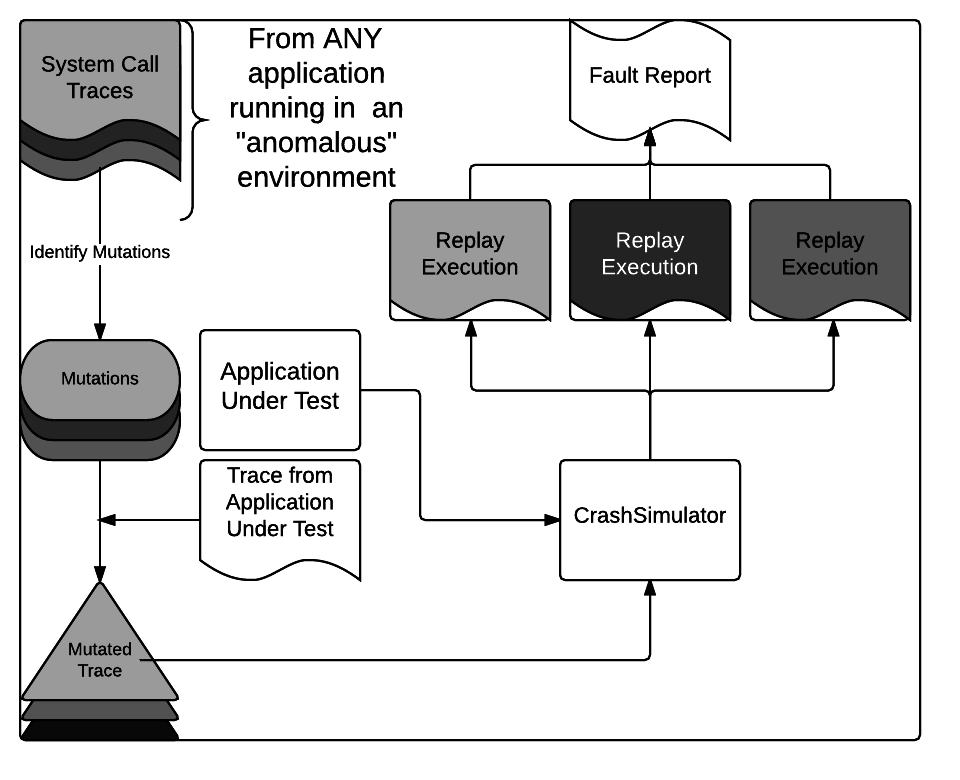
\includegraphics[scale=.5]{Architecture}}
        \caption{\emph{We need a new figure.}}

    \end{figure*}

    \subsection{CrashSimulator's Approach}

    CrashSimulator's testing process is based on two concepts: the encoding of error conditions as a generic
    computational model and the deterministic replay of a system call trace recorded from the application being tested.

    Prior to beginning CrashSimulator's testing process, a set of bad behaviors (which we refer to as anomalies) to test
    for must be identified.  A variety of tools capable of identifying anomalies usable by CrashSimulator already
    exist.  This work relies on NetCheck and CheckAPI for this purpose. NetCheck readily able to identify a wide variety
    of anomalous behaviors related to network communication between one or more hosts. During normal operation, NetCheck
    analyzes a group of input system call traces and attempts to produce a diagnosis for network related
    faults. CheckAPI peforms a similar function by comparing ``behavior of an API implementation to a reference model.''

    Additionally, anomalies can be identified through standard bug hunting techniques.  In this work we constructed
    models that identified bad behavior around moving files from one filesystem to another.  Using these models,
    CrashSimulator was able to identify when applications (nodejs etc.) performed this operation incorrectly.

    Another source of anomalies is the public bug trackers of projects available on the web.  The presence of a bug can
    be defined as a series of system calls then a model that identifies during execution can be constructed.  This can
    be useful in the case of the major, highly publicized bugs that have been found recently.  Similarly, bugs can be
    taken from similar projects in order to expand a project's ``test suite.''

    Once a set of anomalies have been identified, they must be converted to a format that CrashSimulator is able to
    utilize.  This process involves examining the traces containing anomalies in order to identify a series of system
    calls indicative of the presence of the anomaly.  In this work, this series of system calls is encoded as a
    computational model (e.g. a deterministic finite automaton, a push down automaton, etc.) that, when provided with as
    input the system calls made during the course of an execution, can decide whether or the series of system calls is
    present.

    For example, if an anomaly is identified in a web server application, this behavior can likely distilled down to a
    series of system calls indicitive of the anomaly being present.  If this bad behavior is present in other
    network-reliant applications it too can be identified by looking for the same series of system calls.  This series
    of system calls can then be transformed into a computational model as described above.  As another example, consider
    the bugs in Python's shutils that were discussed earlier.  In the case of the ``race condition'' bug, the series of
    system calls indicative of its presence is an application using stat() to check a file, open() to open it, and a
    series of read() and write() calls to copy its contents to the destination without a call to fstat() that to confirm
    that the file was not modified after the initial call to stat().

    The next step in CrashSimulator's testing process is to run CrashSimulator's replay tool against the application
    being tested.  In the simplest case, this involves first recording a system call trace of a ``normal'' execution of
    the application.  This system call trace is replayed -- an operation that allows CrashSimulator to monitor the
    execution utilizing the computational models discussed above.  The reply process consists of CrashSimulator
    launching the application under test as a child process and interceeding in its execution at approprate times in
    order to simulate the results and side effects of any system calls the application makes.  After the repayed
    execution concludes, CrashSimulator able to use the ending state of the models to report whether or not anomalous
    behavior was present.  In the case of the Python shutils race condition, the faulty behavior can be identified using
    a simple python script that calls shutils.move() to move a file between directories located on different storage
    devices.  CrashSimulator is able to identify the bad behavior by replaying a system call trace taken of an
    execution of the Python interpreter while it executes the script in question.

    In a more complex case, CrashSimulator's replay capability can be exploited in order to control execution of the
    application under test in order to force an anomalous condition.  For example, a set of bugs that will be discussed
    later were found by modifying a rename() system call to return a result indicating that the application is
    attempting to move a file across disks -- an operation the system call cannot perform.  In a well behaved
    application, this will trigger an alternative execution path wherein the file is manually copied by the application.
    In a buggy application either this case will be handled incorrectly (i.e. the appliation will fail to perform all of
    the steps required to properly copy a file across devices, a situation caught by well-constructed anomaly models) or
    will not be handled at all, that is, the application will fail eventually because it did not recognize that the call
    to rename was not successful.

    The steps of this process related to constructing the computational models do not need to be repeated.  Instead, the
    models and, if necessary, their associated modifications to the ``normal'' trace can be accumulated into waht
    amounts to a test suite that can be run against any application the CrashSimulator's user is interested in.  This is
    one of CrashSimulator's primary advantages over application-specific test suites or other testing techniques -- the
    upfront work can be performed once and then used repeatedly across any application.

    \paragraph{Active vs. Passive Bugs}

    The set of bugs that CrashSimulator can identify can be broken up into two classes based on what action is necessary
    in order to make them appear.  This work refers to the simplest case as ``passive'' bugs.  These are bugs that can
    be identified by a computational model as it monitors a replayed execution based on an \emph{unmodified} system call
    trace of the application being tested.  That is, the replayed execution exhibits the series of system call
    indiciative of the target anomalous behavior without CrashSimulator having to inject some ``trigger'' behavior from
    a modified version of the trace (e.g. the modifications to the rename() call discussed above).   This work refers to
    the second class of the bug as ``active'' bugs.  In this case, some modification must be made to the trace that is
    going to be replayed in order to coerce execution a targeted execution path where anomalous behavior may be present.
    
    \paragraph{What Can a Test Tell Us?}

    In short, a test can only tell is if an application performs a specific bad behavior in a specific situation.  This
    is in opposition to telling us that an application is bug free in a given situation.  With this in mind, the usual
    approach is to construct a large enough test suite that some desired degree of coverage is achieved.  CrashSimulator
    operates according to this approach as well.  Each injected anomaly can be considered a test case and a set of
    anomalies can be considered a test suite.  The advantage CrashSimulator has over other tools is that these ``tests''
    can be utilized across a variety of applications whereas a traditional test suite is closely coupled to the
    application it tests.  As with traditional tests, CrashSimulator cannot tell us that an applcation is bug free in a
    given situation -- instead it can assert that an application has incorrectly handled a given situation based.

    \paragraph{Classifying Program Behavior}

    For ``active'' bugs, if CrashSimulator injects behavior that \emph{should} necesistate some deviant behavior but the
    application continues along the the same execution path as is recorded in the system call trace then the application
    has not properly handled the injected bejavior.  For example, if CrashSimulator modifies the data structure
    ``returned'' by a call to stat64() such that the target file appears to be a symlink rather than a regular file and
    the application being replayed does not alter its behavior to deal with this fact, the application has not correctly
    handled the injected behavior -- a failing result.  Alternatively, if the application deivates from the behavior
    described in the system call trace driving the replay it is likely that the application is taking some action to
    handle the injected condition -- an indiciation of possibly correct behavior.

    In the case of both ``active'' and ``passive'' bugs, determinations about program behavior can be made based on the
    ending states of any computational models employed during CrashSimulator's replay of the execution.  Part of
    encoding a series of system calls as an appropriate computational model is identifying what states constitute a
    situation where the model ``accepts'' (i.e. asserts as correct) the programs behavior and what states make up a
    situation where the model ``rejects'' (i.e. asserts as incorrect) the programs behavior.

    \subsection{Architecture}
        
    At a high level CrashSimulator is organized into three primary modules. The first module is responsible for
    monitoring a given execution, determining when to inject anomalous behavior, determining whether or not the
    application responded correctly to the injected behavior. The second module is responsible for managing the
    execution of the application under test such that it precisely follows a previously recorded system call trace -- a
    process we refer to as ``replaying'' a system call trace. The third module orchestrates the process of running
    multiple different anomalies against the application under test, much like a unit test suite.
        
    The first step in CrashSimulator's work flow is to identify anomalous behavior in an arbitrary application.
    Currently, this step is accomplished through manual bug hunting and through examination of diagnostic output from
    NetCheck and CheckAPI. CrashSimulator's user examines the system call behavior that resulted in this bad behavior
    and constructs a model that defines what triggers the anomalous behavior and the subsequent ``bad'' system call
    behavior (\emph{Do we need to say something about future work doing this step automatically here?}.
    CrashSimulator's first module operates by using this model to analyzed the system call behavior of the application
    under test(e.g. order, parameters, side effects, return values).
        
    CrashSimulator's second module makes use of the Ptrace facilities built into modern versions of the Linux
    kernel. The aforementioned ``replay'' of a system call trace is achieved by intercepting every system call the
    application makes, preventing the actual system call from being carried out by the kernel (i.e. no-oping out the
    real system call, that is replacing it with a call to getpid()), identifying the matching system call from the
    previously recorded trace, and replicating the return value and side effects such that the application believes that
    the system call it made actually took place. We have found that emulating the post conditions of the system calls an
    application makes results in faithful replay of a previous execution in most cases.

    Replay is important because it allows CrashSimulator to execute an application free from dependencies on things like
    file system contents, network configuration, or communication with other applications....... \emph{need more here
      -Preston}

    All three primary CrashSimulator modules are packaged together and interact with each other at the appropriate times
    without user intervention. At this point, CrashSimulator itself is available as a virtual machine appliance
    compatible with the \emph{Virtual Box} virtual machine hosting software. The reasons for distributing CrashSimulator
    in this manner are threefold. First, this distribution method ensures that all of CrashSimulator's dependences are
    installed and configured appropriately. Second, this method provides an environment for taking system call traces
    that is known to be complete tool-wise and compatible with CrashSimulator. Finally, and most importantly, this
    method provides an environment that is known to be compatible with the details of CrashSimulator's system call
    replay techniques.

    CrashSimulator's source code is available and, while other environments may be untested, it should function
    correctly on any platforms that meet the criteria described above.

    \subsection{System Call Traces and Replay}

        \subsubsection{Why System Call Traces?}

        In order to inject anomalies and monitor program behavior as described above, CrashSimulator needs to have detailed
        interactions with the application under test at some level.  The option of carrying out these interactions at the
        system call level was chosen because for several reasons:

        \paragraph{Tooling}

        Operating at the system call level allows this work to take advantage of two key pieces of tooling that already
        exist in mature form on Linux.  The first is ptrace. Ptrace is a process manipulation interface provided by the
        Linux kernel whose primary use case is debugger development.  This work leverages ptrace in order to start and
        stop execution of a process as well as read and write the contents of the processes registers and memory.  Using
        these operations allows CrashSimulator to pause execution before and after each system call an application makes
        in order to manage execution and inject anomalies where appropriate.

        This CrashSimulator also relies on system call traces recorded using strace.  The strace system call trace format is
        extensive and captures the parameters, return values, and side effects of each system call an application makes.
        Such a record provides CrashSimulator with all the information needed to direct execution of the application in such
        a way that the contents of the system call trace are faithfully replayed.  It is in this way that system call traces
        act as an interface over an applications execution that used to inject anomalous behavior.

        \paragraph{Removal of language dependence}

        Operating at the system call level means that CrashSimulator is not dependant on a particular programming
        language or runtime.  This means that CrashSimulator does not require any complext language parsing and analysis
        while still posessing many of the benefits of systems that perform such work.  Tools that perform language
        parsing do so in order to craft inputs that specifically exercise target execution paths in an application.
        This work is concerned with issues that arise at the ``interfaces'' between an application and its environment.
        Manipulating system calls allows us to skip the process of generating these inputs in favor of directly
        effecting the behavior we are interested in.

        \paragraph{Identify Issues that Result from an Application's Environment}

        Most current testing strategies are very application-centric.  For example, a black box fuzzer is able to
        identify faults that arise when an application begins processing data it has received from a network
        connection. CrashSimulator, on the other hand, is able to identify issues that arisese from the network connection
        itself.

    \subsubsection{Why Replay Executions?}

    \emph{I need to quit saying ``For Example'' so much -Preston}

    \paragraph{Removal of Dependencies}

    Replaying an execution allows CrashSimulator, in many cases, to completely simulate some aspect of an applications
    environment using the data recorded in a system call trace from a previous application.  For example, if an
    application depends on a file being present in a filesystem, CrashSimulator can intercept calls to read()
    from / write() to this file alleviating the need this file to actually be present during replay executions.

    \paragraph{Control Execution}

    Because it is simulating aspects the application under test's environment, CrashSimulator is able to manipulate the
    data the application receives from these aspects in order to control execution.  This is the key feature that allows
    CrashSimulator to inject anomalous situations into an execution.  For example, by simulating the communications
    between the application under test and another host on a network, CrashSimulator can fragment, modify, or even drop
    data ``incoming'' from the simulated remote host in order to determine whether or not the application appropriately
    handles the situation. 